Una vez seleccionado el simulador base y definida la biblioteca de compresión a emplear, el siguiente paso consiste en establecer una arquitectura
de simulación que permita introducir compresión sin pérdida sin alterar la semántica del simulador de estado completo. En esta sección se presenta
una propuesta de diseño en niveles de abstracción, pensada para ser reutilizable en cualquier simulador tipo Schrödinger cuyo estado cuántico se
represente como un vector de amplitudes complejas en doble precisión.

\begin{figure}[H]
    \centering
    \caption{Arquitectura por bloques para la integración de compresión sin pérdida en simuladores cuánticos tipo Schrödinger}
    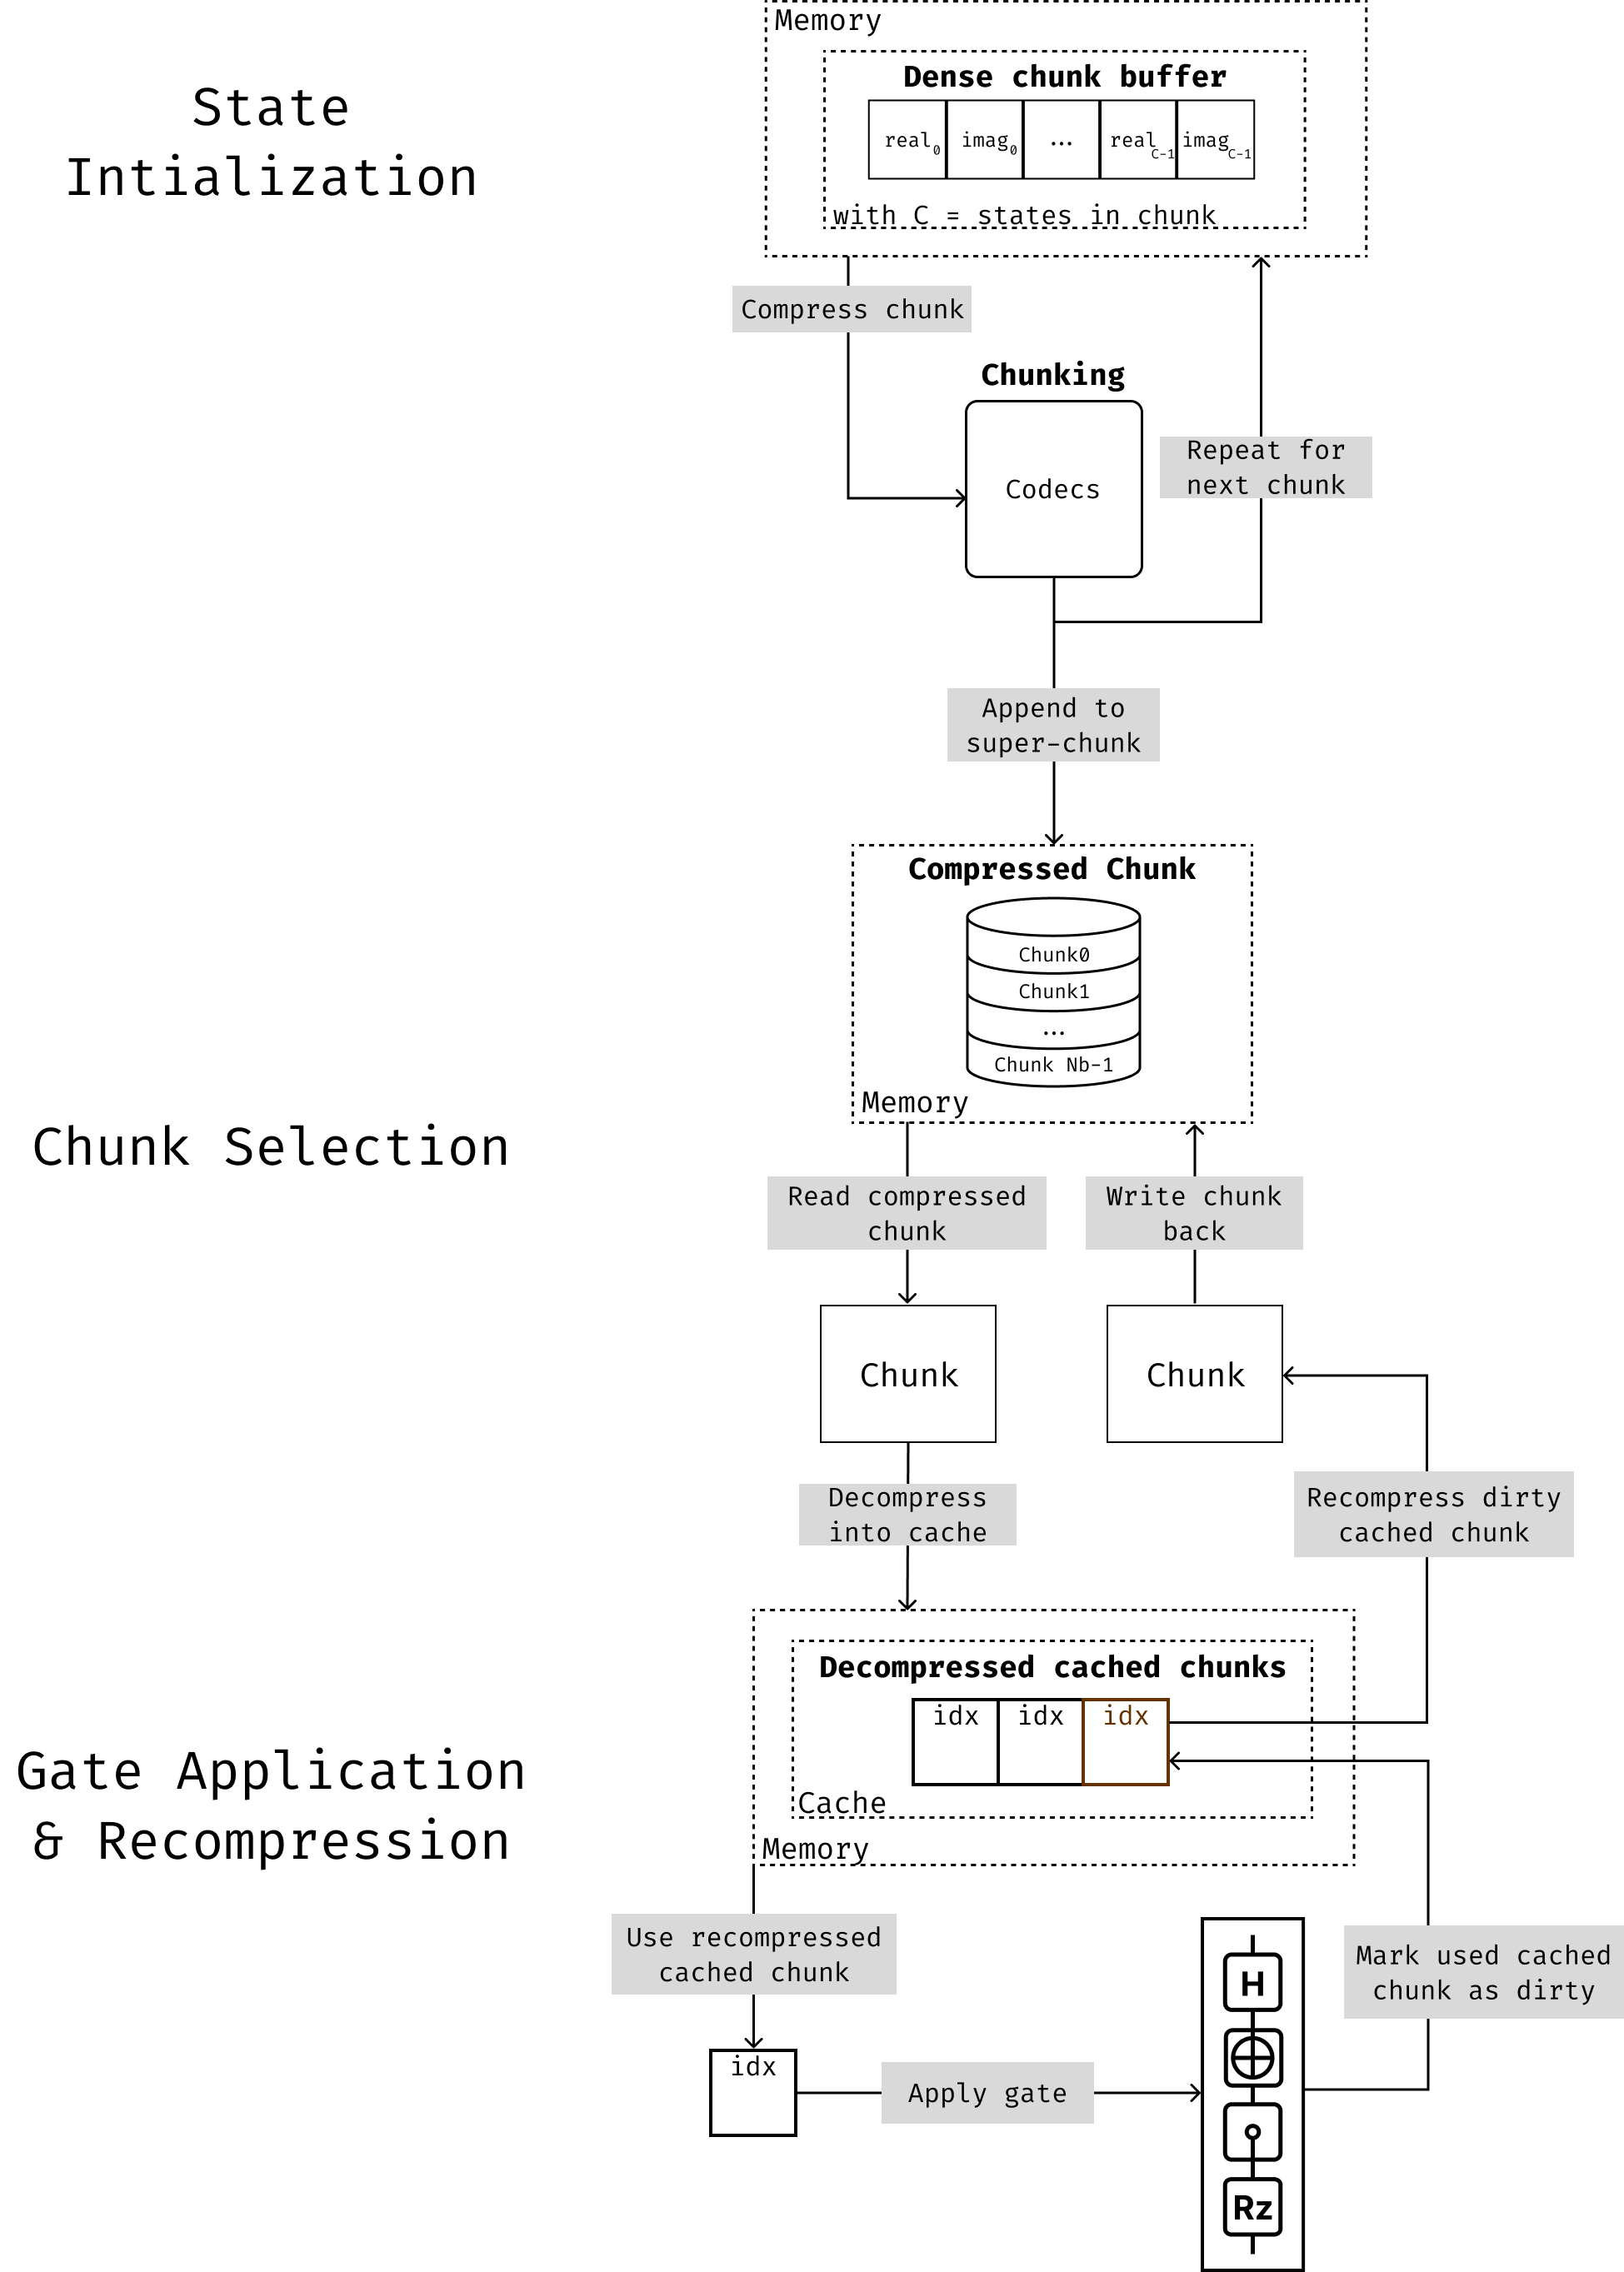
\includegraphics[height=1.3\textwidth]{images/development-architecture.png}
    \label{fig:simulation-design-architecture}
\end{figure}
